% Author: Sven Jacobs
% Content: Code generating the alternative causal graph
% OSE data science, Prof. Dr. Philipp Eisenhauer | Summer 2021, M.Sc. Economics, Bonn University

\documentclass[tikz, margin = 10pt]{standalone}

\usetikzlibrary{arrows.meta}
\tikzset{-Latex, bidirected/.style = {Latex-Latex, dashed, fill = white, overlay}}

\begin{document}

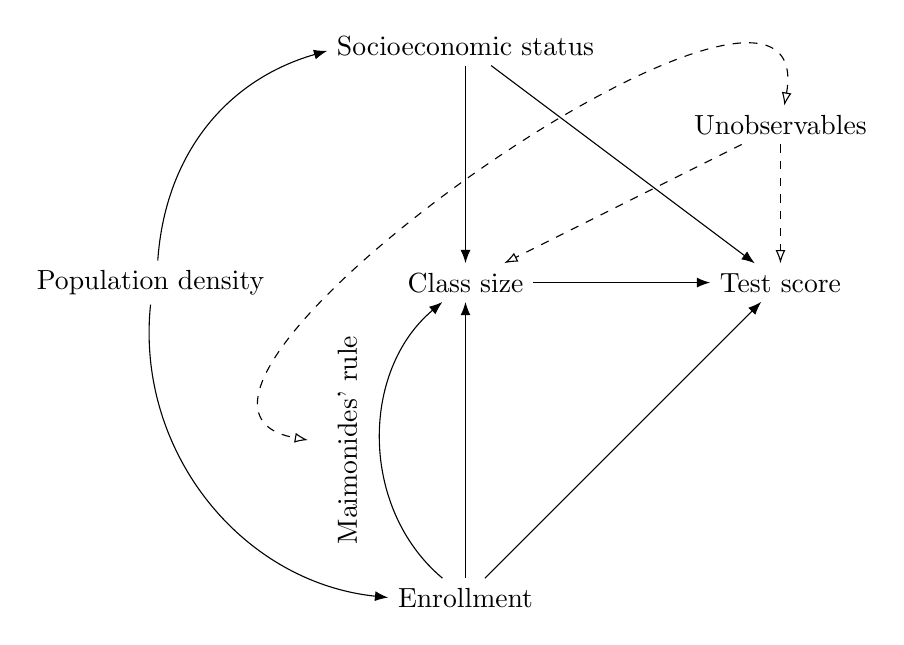
\begin{tikzpicture}
	
	\node (1) at (0, 0) {Class size};
	\node (2) at (0, 3) {Socioeconomic status};
	\node (3) at (0, -4) {Enrollment};
	\node (4) at (4, 0) {Test score};
	\node (5) at (-4, 0) {Population density};
	\node (6) at (4, 2) {Unobservables};
	
	\path (2) edge (1);
	\path (3) edge (1);
	\path (1) edge (4);
	\path (2) edge (4);
	\path (3) edge (4);
	
	\path[fill = white] (6) edge[dashed] (1);
	\path[fill = white] (6) edge[dashed] (4);
	
	\path (5) edge[bend left = 35] (2);
	\path (5) edge[bend right = 45] (3);
	\path (3) edge[bend left = 50] node[sloped, above = 5pt] {Maimonides' rule} (1);
	
	\path[bidirected] (6) edge[bend right = 135] (-2, -2); 
	
\end{tikzpicture}
	
\end{document}